\section{Evaluation}

\begin{table*}[]
\centering
\caption{Averaged performance over 30 trials on incident type prediction}
\tiny
\begin{tabular}{||c|cccc|cccc|cccc||}
\hline
Incident Type & \multicolumn{4}{c|}{Minor Crash Report}                                                                                                    & \multicolumn{4}{c|}{Lost or Stolen Property}                                                                                               & \multicolumn{4}{c||}{Aggressive Drivers}                                                                                                    \\ \hline\hline
Metric        & \multicolumn{1}{c|}{Precision}         & \multicolumn{1}{c|}{Recall}            & \multicolumn{1}{c|}{F-1}              & Accuracy         & \multicolumn{1}{c|}{Precision}         & \multicolumn{1}{c|}{Recall}            & \multicolumn{1}{c|}{F-1}              & Accuracy         & \multicolumn{1}{c|}{Precision}         & \multicolumn{1}{c|}{Recall}            & \multicolumn{1}{c|}{F-1}              & Accuracy         \\ \hline
LSTM          & \multicolumn{1}{c|}{40.00\%}           & \multicolumn{1}{c|}{96.00\%}           & \multicolumn{1}{c|}{56.47\%}          & 42.19\%          & \multicolumn{1}{c|}{0.00\%}            & \multicolumn{1}{c|}{0.00\%}            & \multicolumn{1}{c|}{0.00\%}           & 00.00\%          & \multicolumn{1}{c|}{36.84\%}           & \multicolumn{1}{c|}{84.62\%} & \multicolumn{1}{c|}{53.85\%}          & 62.50\%          \\ \hline
CNN           & \multicolumn{1}{c|}{66.67\%}           & \multicolumn{1}{c|}{88.00\%}           & \multicolumn{1}{c|}{75.86\%}          & 78.13\%          & \multicolumn{1}{c|}{\textbf{93.75\%}} & \multicolumn{1}{c|}{75.00\%}  & \multicolumn{1}{c|}{85.71\%}          & 83.75\%          & \multicolumn{1}{c|}{93.33\%} & \multicolumn{1}{c|}{57.14\%}           & \multicolumn{1}{c|}{72.72\%}          & 60.61\%          \\ \hline
RCNN          & \multicolumn{1}{c|}{85.71\%}           & \multicolumn{1}{c|}{96.00\%}  & \multicolumn{1}{c|}{90.57\%}          & 92.18\%          & \multicolumn{1}{c|}{77.78\%}           & \multicolumn{1}{c|}{87.50\%}           & \multicolumn{1}{c|}{82.35\%}          & 80.63\%          & \multicolumn{1}{c|}{66.67\%}           & \multicolumn{1}{c|}{57.14\%}           & \multicolumn{1}{c|}{61.54\%}          & 64.38\%          \\ \hline
RNN           & \multicolumn{1}{c|}{54.29\%}           & \multicolumn{1}{c|}{76.00\%}           & \multicolumn{1}{c|}{63.33\%}          & 65.63\%          & \multicolumn{1}{c|}{42.86\%}           & \multicolumn{1}{c|}{37.50\%}           & \multicolumn{1}{c|}{40.00\%}          & 41.88\%          & \multicolumn{1}{c|}{37.50\%}           & \multicolumn{1}{c|}{85.71\%}           & \multicolumn{1}{c|}{52.17\%}          & 65.63\%          \\ \hline
SelfAtten     & \multicolumn{1}{c|}{85.19\%}           & \multicolumn{1}{c|}{92.00\%}           & \multicolumn{1}{c|}{88.46\%}          & 90.63\%          & \multicolumn{1}{c|}{80.00\%}           & \multicolumn{1}{c|}{\textbf{97.98\%}} & \multicolumn{1}{c|}{88.89\%}          & 93.75\%          & \multicolumn{1}{c|}{80.00\%}           & \multicolumn{1}{c|}{57.14\%}           & \multicolumn{1}{c|}{66.67\%}          & 67.50\%          \\ \hline
Attention     & \multicolumn{1}{c|}{76.32\%}           & \multicolumn{1}{c|}{87.88\%}           & \multicolumn{1}{c|}{91.69\%}          & 79.69\%          & \multicolumn{1}{c|}{62.50\%}           & \multicolumn{1}{c|}{62.50\%}           & \multicolumn{1}{c|}{62.50\%}          & 61.25\%          & \multicolumn{1}{c|}{60.00\%}           & \multicolumn{1}{c|}{42.56\%}           & \multicolumn{1}{c|}{50.00\%}          & 81.25\%          \\ \hline
Bert          & \multicolumn{1}{c|}{93.06\%}  & \multicolumn{1}{c|}{\textbf{97.10\%}}           & \multicolumn{1}{c|}{95.04\%} & 95.76\% & \multicolumn{1}{c|}{88.00\%}           & \multicolumn{1}{c|}{95.20\%}           & \multicolumn{1}{c|}{91.50\%} & 95.60\% & \multicolumn{1}{c|}{93.75\%}  & \multicolumn{1}{c|}{90.91\%}           & \multicolumn{1}{c|}{92.31\%} & 93.75\% \\ \hline
\textbf{Auto311}          & \multicolumn{1}{c|}{\textbf{97.10\%}}  & \multicolumn{1}{c|}{94.37\%}           & \multicolumn{1}{c|}{\textbf{95.71\%}} & \textbf{96.34\%} & \multicolumn{1}{c|}{90.91\%}           & \multicolumn{1}{c|}{95.20\%}           & \multicolumn{1}{c|}{\textbf{93.00\%}} & \textbf{96.70\%} & \multicolumn{1}{c|}{\textbf{93.75\%}}  & \multicolumn{1}{c|}{\textbf{93.75\%}}           & \multicolumn{1}{c|}{\textbf{93.75\%}} & \textbf{94.94\%} \\ \hline\hline
Incident Type & \multicolumn{4}{c|}{Check Welfare}                                                                                                         & \multicolumn{4}{c|}{Damaged Property}                                                                                                      & \multicolumn{4}{c||}{Noise Violation}                                                                                                       \\ \hline\hline
Metric        & \multicolumn{1}{c|}{Precision}         & \multicolumn{1}{c|}{Recall}            & \multicolumn{1}{c|}{F-1}              & Accuracy         & \multicolumn{1}{c|}{Precision}         & \multicolumn{1}{c|}{Recall}            & \multicolumn{1}{c|}{F-1}              & Accuracy         & \multicolumn{1}{c|}{Precision}         & \multicolumn{1}{c|}{Recall}            & \multicolumn{1}{c|}{F-1}              & Accuracy         \\ \hline
LSTM          & \multicolumn{1}{c|}{46.88\%}           & \multicolumn{1}{c|}{\textbf{97.54\%}} & \multicolumn{1}{c|}{82.35\%}          & 46.88\%          & \multicolumn{1}{c|}{0.00\%}            & \multicolumn{1}{c|}{0.00\%}            & \multicolumn{1}{c|}{0.00\%}           & 0.00\%          & \multicolumn{1}{c|}{0.00\%}            & \multicolumn{1}{c|}{0.00\%}            & \multicolumn{1}{c|}{0.00\%}           & 0.00\%          \\ \hline
CNN           & \multicolumn{1}{c|}{68.18\%}           & \multicolumn{1}{c|}{96.54\%} & \multicolumn{1}{c|}{81.08\%}          & 78.13\%          & \multicolumn{1}{c|}{25.00\%}           & \multicolumn{1}{c|}{66.67\%} & \multicolumn{1}{c|}{40.00\%}          & 25.00\%          & \multicolumn{1}{c|}{66.67\%} & \multicolumn{1}{c|}{28.57\%}           & \multicolumn{1}{c|}{44.44\%}          & 34.38\%          \\ \hline
RCNN          & \multicolumn{1}{c|}{73.64\%}           & \multicolumn{1}{c|}{93.33\%}           & \multicolumn{1}{c|}{82.35\%}          & 81.25\%          & \multicolumn{1}{c|}{93.75\%} & \multicolumn{1}{c|}{62.50\%}           & \multicolumn{1}{c|}{76.92\%}          & 70.61\%          & \multicolumn{1}{c|}{96.77\%} & \multicolumn{1}{c|}{71.43\%}  & \multicolumn{1}{c|}{83.33\%} & 93.75\% \\ \hline
RNN           & \multicolumn{1}{c|}{73.33\%}           & \multicolumn{1}{c|}{73.33\%}           & \multicolumn{1}{c|}{73.33\%}          & 75.00\%          & \multicolumn{1}{c|}{31.58\%}           & \multicolumn{1}{c|}{75.00\%}           & \multicolumn{1}{c|}{44.44\%}          & 53.13\%          & \multicolumn{1}{c|}{96.77\%} & \multicolumn{1}{c|}{71.43\%}  & \multicolumn{1}{c|}{83.33\%} & 93.75\% \\ \hline
SelfAtten     & \multicolumn{1}{c|}{82.35\%}           & \multicolumn{1}{c|}{93.33\%}           & \multicolumn{1}{c|}{87.50\%}          & 87.50\%          & \multicolumn{1}{c|}{71.43\%}           & \multicolumn{1}{c|}{62.50\%}           & \multicolumn{1}{c|}{66.67\%}          & 64.38\%          & \multicolumn{1}{c|}{60.00\%}           & \multicolumn{1}{c|}{42.86\%}           & \multicolumn{1}{c|}{50.00\%}          & 51.25\%          \\ \hline
Attention     & \multicolumn{1}{c|}{45.83\%}           & \multicolumn{1}{c|}{64.71\%}           & \multicolumn{1}{c|}{53.66\%}          & 50.31\%          & \multicolumn{1}{c|}{75.00\%} & \multicolumn{1}{c|}{37.50\%}           & \multicolumn{1}{c|}{54.55\%}          & 54.38\%          & \multicolumn{1}{c|}{57.14\%} & \multicolumn{1}{c|}{42.86\%}           & \multicolumn{1}{c|}{60.00\%}          & 57.50\%          \\ \hline
Bert          & \multicolumn{1}{c|}{93.10\%}  & \multicolumn{1}{c|}{87.10\%}           & \multicolumn{1}{c|}{90.00\%} & 90.63\% & \multicolumn{1}{c|}{80.00\%} & \multicolumn{1}{c|}{87.88\%}           & \multicolumn{1}{c|}{88.89\%} & 94.12\% & \multicolumn{1}{c|}{96.77\%} & \multicolumn{1}{c|}{71.43\%}  & \multicolumn{1}{c|}{83.33\%} & 93.75\% \\ \hline
\textbf{Auto311}          & \multicolumn{1}{c|}{\textbf{93.10\%}}  & \multicolumn{1}{c|}{87.10\%}           & \multicolumn{1}{c|}{\textbf{90.00\%}} & \textbf{90.63\%} & \multicolumn{1}{c|}{88.89\%}           & \multicolumn{1}{c|}{\textbf{99.01\%}}           & \multicolumn{1}{c|}{\textbf{94.12\%}} & \textbf{96.88\%} & \multicolumn{1}{c|}{\textbf{96.77\%}}  & \multicolumn{1}{c|}{\textbf{71.43\%}}           & \multicolumn{1}{c|}{\textbf{83.33\%}} & \textbf{93.75\%} \\ \hline\hline

Incident Type & \multicolumn{4}{c|}{Roadway Hazard}                                                                                                        & \multicolumn{4}{c|}{Abandoned Vehicles}                                                                                                    & \multicolumn{4}{c||}{Drug or Prostitution Activity}                                                                                         \\ \hline\hline
Metric        & \multicolumn{1}{c|}{Precision}         & \multicolumn{1}{c|}{Recall}            & \multicolumn{1}{c|}{F-1}              & Accuracy         & \multicolumn{1}{c|}{Precision}         & \multicolumn{1}{c|}{Recall}            & \multicolumn{1}{c|}{F-1}              & Accuracy         & \multicolumn{1}{c|}{Precision}         & \multicolumn{1}{c|}{Recall}            & \multicolumn{1}{c|}{F-1}              & Accuracy         \\ \hline
LSTM          & \multicolumn{1}{c|}{46.88\%}           & \multicolumn{1}{c|}{83.33\%} & \multicolumn{1}{c|}{63.83\%}          & 46.88\%          & \multicolumn{1}{c|}{52.94\%}           & \multicolumn{1}{c|}{\textbf{90.10\%}} & \multicolumn{1}{c|}{69.23\%}          & 60.00\%          & \multicolumn{1}{c|}{50.00\%}           & \multicolumn{1}{c|}{42.86\%}           & \multicolumn{1}{c|}{46.15\%}          & 50.00\%          \\ \hline
CNN           & \multicolumn{1}{c|}{70.00\%}           & \multicolumn{1}{c|}{93.33\%}           & \multicolumn{1}{c|}{80.00\%}          & 78.13\%          & \multicolumn{1}{c|}{45.00\%}           & \multicolumn{1}{c|}{81.08\%} & \multicolumn{1}{c|}{62.07\%}          & 45.00\%          & \multicolumn{1}{c|}{22.22\%}           & \multicolumn{1}{c|}{28.57\%}           & \multicolumn{1}{c|}{25.00\%}          & 14.29\%          \\ \hline
RCNN          & \multicolumn{1}{c|}{86.67\%}           & \multicolumn{1}{c|}{86.67\%}           & \multicolumn{1}{c|}{86.67\%}          & 87.50\%          & \multicolumn{1}{c|}{21.43\%}           & \multicolumn{1}{c|}{33.33\%}           & \multicolumn{1}{c|}{26.09\%}          & 15.00\%          & \multicolumn{1}{c|}{22.22\%}           & \multicolumn{1}{c|}{28.57\%}           & \multicolumn{1}{c|}{25.00\%}          & 14.29\%          \\ \hline
RNN           & \multicolumn{1}{c|}{65.00\%}           & \multicolumn{1}{c|}{84.62\%}           & \multicolumn{1}{c|}{74.29\%}          & 71.88\%          & \multicolumn{1}{c|}{25.00\%}           & \multicolumn{1}{c|}{33.33\%}           & \multicolumn{1}{c|}{28.57\%}          & 25.00\%          & \multicolumn{1}{c|}{25.00\%}           & \multicolumn{1}{c|}{28.57\%}           & \multicolumn{1}{c|}{26.67\%}          & 21.43\%          \\ \hline
SelfAtten     & \multicolumn{1}{c|}{76.47\%}           & \multicolumn{1}{c|}{86.36\%}           & \multicolumn{1}{c|}{81.25\%}          & 81.25\%          & \multicolumn{1}{c|}{8.33\%}            & \multicolumn{1}{c|}{11.11\%}           & \multicolumn{1}{c|}{9.52\%}           & 5.00\%           & \multicolumn{1}{c|}{30.00\%}           & \multicolumn{1}{c|}{42.86\%}           & \multicolumn{1}{c|}{35.29\%}          & 21.43\%          \\ \hline
Attention     & \multicolumn{1}{c|}{68.18\%}           & \multicolumn{1}{c|}{\textbf{96.54\%}} & \multicolumn{1}{c|}{81.08\%}          & 78.12\%          & \multicolumn{1}{c|}{66.67\%}           & \multicolumn{1}{c|}{66.67\%}           & \multicolumn{1}{c|}{66.67\%}          & 70.00\%          & \multicolumn{1}{c|}{55.56\%}           & \multicolumn{1}{c|}{71.43\%}           & \multicolumn{1}{c|}{62.50\%}          & 57.14\%          \\ \hline
Bert          & \multicolumn{1}{c|}{100.00\%} & \multicolumn{1}{c|}{83.33\%}           & \multicolumn{1}{c|}{90.91\%} & 93.10\% & \multicolumn{1}{c|}{100.00\%} & \multicolumn{1}{c|}{88.89\%}  & \multicolumn{1}{c|}{94.12\%} & 95.00\% & \multicolumn{1}{c|}{85.17\%} & \multicolumn{1}{c|}{100.00\%}  & \multicolumn{1}{c|}{92.40\%} & 92.86\% \\ \hline
\textbf{Auto311}          & \multicolumn{1}{c|}{\textbf{100.00\%}} & \multicolumn{1}{c|}{83.33\%}           & \multicolumn{1}{c|}{\textbf{90.91\%}} & \textbf{93.10\%} & \multicolumn{1}{c|}{\textbf{100.00\%}} & \multicolumn{1}{c|}{88.89\%}  & \multicolumn{1}{c|}{\textbf{94.12\%}} & \textbf{95.00\%} & \multicolumn{1}{c|}{\textbf{85.17\%}} & \multicolumn{1}{c|}{\textbf{100.00\%}}  & \multicolumn{1}{c|}{\textbf{92.40\%}} & \textbf{92.86\%} \\ \hline
\end{tabular}
\label{tab:classification}
\end{table*}

% \subsection{Evaluation Setups}

Experiments assess the performance of (1) confidence-guided incident prediction, (2) confidence-guided itemization, and (3) the overall system. Our dataset includes 11,796 non-emergency calls from the DEC in Nashville, TN. Metrics for incident type prediction are precision, recall, F1, and accuracy. The newly introduced text comparison method evaluates itemization module outputs. The experiments were run on a machine with 2.50GHz CPU, 32GB memory, and Nvidia GeForce RTX 3080Ti GPU.

% Key aspects are the multi-faceted evaluation of prediction, itemization, and end-to-end modules, using real-world call data.

% Our dataset is provided by the local government and the local call center. It consists of 11,796 non-emergency calls in total. The metrics we used to evaluate the incident type prediction module are precision, recall, f-1 score, and accuracy. We use the newly introduced text comparison method to evaluate the textual outputs from the information itemization module and the annotated answers. We design our experiments mainly to discuss (1) the performance of confidence-guided incident type prediction, (2) the performance of confidence-guided information itemization, and (3) the performance of Auto311 at a system level. The experiments were run on a machine with 2.50GHz CPU, 32GB memory, and Nvidia GeForce RTX 3080Ti GPU.

\subsection{Confidence-guided Incident Type Prediction}

This section aims to evaluate Auto311's performance on incident type prediction. Baselines use various neural networks like LSTM, CNN, RCNN, Self-Attention, Bahdanau's Attention, and BERT \cite{hochreiter1997long, kim2014convolutional, lai2015recurrent, vaswani2017attention, bahdanau2014neural, wolf2019huggingface}(see Table \ref{tab:classification}). We include 9 categories due to the page limit (full results including standard deviation stats in Appendix). Experiments comprehensively assess prediction with different model architectures on real call data.


% This section aims to evaluate Auto311's performance on incident type prediction. To fully evaluate the module, we implement different backend neural network structures as baselines, like LSTM \cite{hochreiter1997long}, CNN \cite{kim2014convolutional}, RCNN \cite{lai2015recurrent}, Self-Attention \cite{vaswani2017attention}, Bahdanau's Attention \cite{bahdanau2014neural}, and BERT \cite{wolf2019huggingface}, see performances in \ref{tab:classification}. Here we only include 9 categories due to the page limit (see comprehensive results in the Appendix).

Analysis shows traditional models like CNN perform poorly, with just 62.99\% average F1 on 9 types. Transcription diversity from varied callers increases task complexity (e.g., different speaking habits), challenging learning without prior knowledge. BERT surpasses other models, with 92.54\% average F1 and 100\% max across all 11 types. Leveraging BERT's pre-trained weights and confidence guidance, Auto311 further improves BERT F1 from 91.50\% to 93.00\% for lost/stolen cases. Results demonstrate prediction difficulties due to call diversity and Auto311's enhancements over BERT using confidence scoring.

% Analysis of the results initially reveals that traditional text classification neural network models demonstrate poor performance across most incident types, e.g., CNN for text classification only yields an average 62.99\% F-1 score on those 9 incident types. This suboptimal outcome comes from the diverse formats of the audio transcriptions, which originate from varied callers and consequently exhibit substantial variations in length, vocabulary, and grammar. These differences increase classification task complexity, posing difficulties for traditional models to learn without prior knowledge. Additionally, comprehensive results demonstrate the BERT model surpasses other models across all 11 incident types, achieving an average F-1 score of 92.54\% and a maximum of 100.00\%. Additionally, leveraging prior knowledge furnished by pre-trained BERT weights, Auto311 even obtains improvements with the enhancement from the confidence guidance, e.g., boosting  BERT's F-1 score from 91.50\% to 93.00\% when dealing with lost or stolen cases.

% After analyzing the results, we first notice that traditional text classification neural network models do not perform well in most incident types. The reason behind this is the diverse formats of audio transcriptions. These transcriptions come from various callers, leading to significant variations in length, vocabulary, and grammar. These differences increase the complexity of the classification task, making it challenging for traditional models to learn without prior knowledge. Second, in the comprehensive results, the BERT model outperforms other models in all 11 incident types with an average F-1 score of 92.54\%, highest 100.00\%. With the prior knowledge provided in the pre-trained BERT weights, the downstream classification layers show a better overall performance in all incident types.

% \textit{In summary, results show effective incident type prediction, with BERT backend giving top F1 scores. Confidence guidance further improves performance. This demonstrates high-quality multi-label classification for calls with multiple incident types. The prediction module effectively dispatches calls to all relevant types.}


\textit{In summary, based on the results, Auto311 effectively dispatches the ongoing call to the given incident types. In terms of F-1 score, the BERT backend has the most competitive results. Confidence guidance further improves performance.}

% We also test the ability of our multi-layer classification structure when faced with situations where (1) the caller switches the incident type and (2) the caller includes more than one incident type during the call.

% The objective is to demonstrate the performance of the classification model. This will be achieved through (1) the accuracy of our model of some direct caller utterances and (2) the ability to dynamically change if the caller switches the intention during the call.

% \subsection{Validating Proposed Metric for Text Comparison}

% We conduct an evaluation to assess the effectiveness of our proposed text comparison metric, targeting on the question ``\textbf{How does this new text comparison work in this specific scenario?}''. For this evaluation, we manually selected three distinct groups of text pairs:
% \begin{itemize}
%     \item \textbf{Group one} consists of text pairs that are entirely dissimilar, for instance, ``65 South exit 92'' and ``Silver Camaro.'' These pairs serve as a benchmark to evaluate how well the metric can discern vastly different information.
%     \item \textbf{Group two} comprises pairs that exhibit slight differences in their content, but these discrepancies are not significant enough to significantly impact the dispatcher's decision-making process. For example, pairs like ``an SUV type truck'' and ``It's like an SUV type truck, maybe a Tahoe'' fall under this category.
%     \item \textbf{Group three} contains pairs with identical or highly similar information, which are relevant for dispatchers to complete internal reports. Examples of such pairs include ``on the West End Ave'' and ``West End Ave.''
% \end{itemize}

% To test the consistency scores, we utilize traditional metrics like BLEU \cite{papineni2002bleu}, Damerau–Levenshtein Distance (DLD) \cite{damerau1964technique}, and ROUGE \cite{lin-2004-rouge}, in addition to our modified metric. The evaluation aims to compare how each metric performs in distinguishing differences and similarities within the text pairs across these distinct groups. This analysis will provide valuable insights into the efficacy of our proposed metric compared to established text comparison metrics.

% \begin{figure}[t]
%     \centering
%     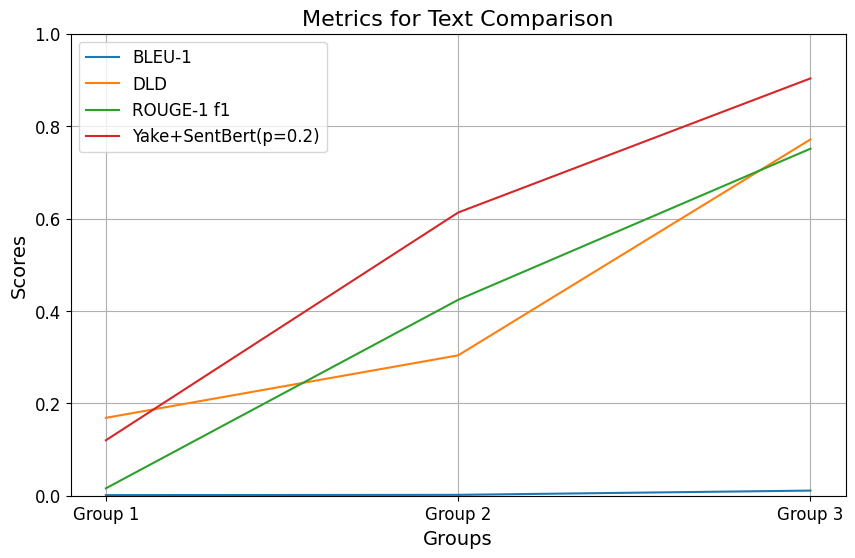
\includegraphics[width=0.45\textwidth]{figures/line-graph.png}
%     \caption{Metric for Text Comparison}
%     \label{fig:textcompare}
%     \vspace{-0.5cm}
% \end{figure}

% Analysis of the plot reveals certain transitional metrics display an upward trend while failing to furnish a fair assessment. The ideal metric yields low scores for group one pair comparisons and high scores for group three pairs. As Figure \ref{fig:textcompare} displays, although exhibiting increased scores from group one to group three, DLD and ROUGE do not account for the robust correlations among text pairs in group three.

% % From analyzing the plot, it is clear that some of the transitional metrics exhibit an upward trend, yet they do not provide a just assessment score. Ideally, we require a metric that yields a low score when comparing group one pairs and a high score when comparing group three pairs. The plot displays in figure \ref{fig:textcompare} reveals that DLD and ROUGE, despite their increasing scores from group 1 to group 3, fail to account for the high correlations among text pairs in group 3. 

% \textit{Ultimately, from the results, it indicates our proposed text comparison metric proves more effective in assessing texts for consistency in this non-emergency dispatching scenario.}

% % The objective is to demonstrate the effectiveness of the text comparison method we propose. We ask dispatchers to (1) evaluate the consistency among a list of texts in a real-world dispatching task, (2) compare our metric with their score, and (3) ask them if the scores make more sense.


\subsection{Confidence-guided Information Itemization}

This experimental setup assesses the performance of the information itemization module of Auto311 using various backends (DistilBERT, BERT, RoBERTa, LongFormer, BigBird \cite{sanh2019distilbert, beltagy2020longformer, zaheer2020big}) and benchmarks (SQuAD, CUAD, TriviaQA \cite{rajpurkar2016squad, rajpurkar2018know, hendrycks2021cuad, joshi2017triviaqa}) and compares it to large language models (LLMs) like GPT3.5 and 4\footnote{Prompt: ``\textit{I will provide context and a set of questions. Please respond to the questions using exact quotes from the context. Your answers should be concise and comprehensive. Context: ...; Question Set: ...''}}, with results in Table \ref{tab:informationextraction}. We utilize our consistency score in this evaluation. Two types of data samples are evaluated for performance: random test samples from archived data (collected by the end of 2022) and the latest data samples (collected from the beginning of 2023) from the call center. Recognizing that city-related information evolves (e.g., new places, activities), we simulate Auto311's usage under knowledge evolution by assessing performance on the latest data samples. Furthermore, we assess Auto311's performance in information itemization when queried with various fields, encompassing basic fields, less specific fields, and more specific fields. Basic fields include essential data like incident location, less specific fields cover descriptors like vehicle and human/suspect descriptions, and more specific fields pertain to incident-specific details such as the timing of the incident (DamagedProperty-when).

% This experimental setup assesses the performance of the information itemization module. We evaluate Auto311's performance in information itemization across various backends (DistilBERT, BERT, RoBERTa, LongFormer, BigBird \cite{sanh2019distilbert, beltagy2020longformer, zaheer2020big}) pre-trained on benchmark datasets (SQuAD, CUAD, TriviaQA \cite{rajpurkar2016squad, rajpurkar2018know, hendrycks2021cuad, joshi2017triviaqa}). Additionally, we compare it with large language models (LLMs) such as GPT3.5 and GPT4 variants\footnote{Prompt: ``\textit{I will provide context and a set of questions. Please respond to the questions using exact quotes from the context. Your answers should be concise and comprehensive.''}}, see results in Table \ref{tab:informationextraction}. We utilize our consistency score in this evaluation. Two types of data samples are evaluated for performance: randomly selected test samples from archived data (collected by the end of 2022) and the latest available data samples (collected from the beginning of 2023) from the local call center. Recognizing that city-related information evolves over time (e.g., new places, activities), we simulate Auto311's usage under knowledge evolution by assessing performance on the latest data samples. Furthermore, we assess Auto311's performance in information itemization when queried with various fields, encompassing basic fields, less specific fields, and more specific fields. Basic fields encompass essential information collected in every call, such as the incident's location (Incident-Location). Less specific fields include descriptors like vehicle description (common in car-related incidents), human/suspect description (relevant in drug-related or welfare check cases), and property description (pertinent to lost-stolen, damaged, or found property cases). More specific fields involve incident-type-specific details, encompassing narrative fields and binary fields like DamagedProperty-when, which inquires about the incident's timing.

% In this experiment setup, we aim to evaluate the performance of the information itemization module. We evaluate Auto311's performance on information itemization with various backends (DistilBERT, BERT, RoBERTa, LongFormer, BigBird \cite{sanh2019distilbert, beltagy2020longformer, zaheer2020big}) pretrained on benchmark datasets (SQuAD, CUAD, TriviaQA \cite{rajpurkar2016squad, rajpurkar2018know, hendrycks2021cuad, joshi2017triviaqa}. We also compare to large language models (LLMs) like ChatGPT variants GPT3.5 and GPT4. Table \ref{tab:informationextraction} shows results. LLMs are constrained to quote words from caller utterances to mimic the extractive process. Our consistency score metric was applied in this evaluation, with two data sample types assessing performance: randomly selected test samples from archived data (collected by the end of 2022) and the latest available data samples (collected from the beginning of 2023) from the local call center. Considering city-related knowledge keeps evolving over time, like newly built places and organized activities, we emulate the usage of Auto311 under knowledge evolution during runtime by also evaluating the performance on the latest data samples. Second, we evaluate Auto311's performance on information itemization when queried with different fields, covering basic fields, less specific fields, and more specific fields. Basic fields include must-collect information in every call, like the location of the incident (Incident-Location). Less specific fields contain fields like vehicle description (likely to appear in most car-related incidents), human/suspect description (likely to appear in drug-pros or check welfare cases), and property description (likely appear in lost-stolen, damaged, or found property cases). More specific fields consist of incident-type-specific fields covering both narrative fields and binary fields like DamagedProperty-when, querying when this incident happened.


% In this experiment setup, we aim to evaluate the performance of the information itemization module. We first evaluate Auto311's performance on information itemization with various backend models (DistilBERT, BERT, RoBERTa \cite{liu2019roberta}, LongFormer \cite{beltagy2020longformer}, BigBird \cite{zaheer2020big}) pretrained on benchmark datasets like SQuAD \cite{rajpurkar2016squad, rajpurkar2018know}, CUAD \cite{hendrycks2021cuad}, TriviaQA \cite{joshi2017triviaqa}. And we also compare its performance with SOTA LLMs (ChatGPT with GPT3.5 \cite{openai_chatgpt_2022}, ChatGPT with GPT4 \cite{openai_gpt4_2023}). The results of this experiment can be found in table \ref{tab:informationextraction}. When comparing with large language models (LLMs), we mandate the provision of answers by quoting callers' exact words. Our consistency score metric was applied in this evaluation, with two data sample types assessing performance: randomly selected test samples from archived data and the latest available data samples from the local call center. The first archived data samples contain previous audio recordings mainly collected by the end of 2022, which Auto311 is trained on. The second latest samples are collected mainly from the beginning of 2023. Considering city-related knowledge keeps evolving over time, we find the latest samples cover time-sensitive information like newly built places and organized activities. Thus, we further emulate the usage of Auto311 under knowledge evolution during runtime. 



% In the competition with LLMs, we have required them to provide answers by quoting the exact words spoken by the caller. Our consistency score metric has been used in this evaluation, and we have used three types of data samples to assess performance. These include test samples randomly selected from the entire dataset, new samples provided by DEC from the latest phone calls, and synthesized samples based on previous question-answer pairs. Batch 3 has been synthesized using a data enrichment algorithm similar to the one used in \cite{chen2022cityspec, chen2023cityspec}.  In addition to batch-wise evaluation, we also test the performance of our module on different question types including unseen specific questions under one certain incident type, e.g., ``what is the color of the vehicle?'' and ``when did this happen?'', see results in Table \ref{tab:different_question_types}.

\begin{table}[h]
\centering
\caption{Performance on information itemization}
\scriptsize
\begin{tabular}{||c|c|c||}
\hline
           & Archived Samples (test) & Latest Samples (runtime)  \\ \hline\hline
DistilBERT-SQuAD2 &  0.5546    & 0.5330                        \\ \hline        
BERT-SQuAD2 &   0.2422   & 0.2791                        \\ \hline
RoBERTa-SQuAD2 &   0.1172   & 0.2581                        \\ \hline
RoBERTa-CUAD &   0.2188   & 0.2378                        \\ \hline
LongFormer-TriviaQA &   0.3260   & 0.1424                        \\ \hline
BigBird-TriviaQA &   0.5289   &     0.5015                    \\ \hline
GPT3.5 (June 2023)     &   0.6343   & 0.6529                         \\ \hline
GPT4 (June 2023)      &   0.6578   & 0.6264                          \\ \hline
\textbf{Auto311}   &   \textbf{0.9329}   & \textbf{0.8605}          \\ \hline
\end{tabular}
\label{tab:informationextraction}
\end{table}

\begin{table*}[t]
\centering
\caption{Auo311's performance on different fields}
\scriptsize
\begin{tabular}{||c|ccccccccc||}
\hline
                  & \multicolumn{3}{c|}{Basic Fields}                                                                                                                                                                                                                                                                                           & \multicolumn{6}{c||}{Less Specific Feilds}                                                                                                                                                                                  \\ \hline\hline
                  & \multicolumn{1}{c|}{Incident-Location}                                                                & \multicolumn{1}{c|}{Caller-Name}                                                                           & \multicolumn{1}{c|}{Caller-Phone \#}                                                                   & \multicolumn{2}{c|}{Vehicle Description}                                       & \multicolumn{2}{c|}{Human/Suspect Description}                                 & \multicolumn{2}{c||}{Property Descritpion}                \\ \hline
w/o Conf Guide    & \multicolumn{1}{c|}{0.9035}                                                                           & \multicolumn{1}{c|}{0.9478}                                                                                & \multicolumn{1}{c|}{1.0000}                                                                            & \multicolumn{2}{c|}{0.8538}                                                    & \multicolumn{2}{c|}{0.9678}                                                    & \multicolumn{2}{c||}{0.9512}                              \\ \hline
w/ Conf Guide     & \multicolumn{1}{c|}{\textbf{0.9631}}                                                                  & \multicolumn{1}{c|}{\textbf{0.9962}}                                                                       & \multicolumn{1}{c|}{\textbf{1.0000}}                                                                   & \multicolumn{2}{c|}{\textbf{0.9104}}                                           & \multicolumn{2}{c|}{\textbf{1.0000}}                                           & \multicolumn{2}{c||}{\textbf{1.0000}}                     \\ \hline\hline
                  & \multicolumn{9}{c|}{More Specific Fields}                                                                                                                                                                                                                                                                                                                                                                                                                                                                                                                \\ \hline\hline
\multirow{2}{*}{} & \multicolumn{1}{c|}{\multirow{2}{*}{\begin{tabular}[c]{@{}c@{}}DamagedProperty\\ -When\end{tabular}}} & \multicolumn{1}{c|}{\multirow{2}{*}{\begin{tabular}[c]{@{}c@{}}AggressiveDriver\\ -Behavior\end{tabular}}} & \multicolumn{1}{c|}{\multirow{2}{*}{\begin{tabular}[c]{@{}c@{}}CheckWelfare\\ -Relation\end{tabular}}} & \multicolumn{3}{c|}{\begin{tabular}[c]{@{}c@{}}MinorCrash\\ -BlockTraffic (Y/N)\end{tabular}}                          & \multicolumn{3}{c||}{\begin{tabular}[c]{@{}c@{}}CheckWelfare\\ -InpersonMeet (Y/N)\end{tabular}}   \\ \cline{5-10} 
                  & \multicolumn{1}{c|}{}                                                                                 & \multicolumn{1}{c|}{}                                                                                      & \multicolumn{1}{c|}{}                                                                                  & \multicolumn{1}{c|}{P}                 & \multicolumn{1}{c|}{R}                & \multicolumn{1}{c|}{F-1}              & \multicolumn{1}{c|}{P}                 & \multicolumn{1}{c|}{R}                & F-1              \\ \hline
w/o Conf Guide    & \multicolumn{1}{c|}{0.9045}                                                                           & \multicolumn{1}{c|}{0.8255}                                                                                & \multicolumn{1}{c|}{0.9023}                                                                            & \multicolumn{1}{c|}{66.67\%}          & \multicolumn{1}{c|}{100.00\%}          & \multicolumn{1}{c|}{80.0\%}           & \multicolumn{1}{c|}{83.33\%}           & \multicolumn{1}{c|}{83.33\%}          & 83.33\%          \\ \hline
w/ Conf Guide     & \multicolumn{1}{c|}{\textbf{1.000}}                                                                   & \multicolumn{1}{c|}{\textbf{0.9164}}                                                                       & \multicolumn{1}{c|}{\textbf{0.9855}}                                                                   & \multicolumn{1}{c|}{\textbf{88.89\%}} & \multicolumn{1}{c|}{\textbf{100.00\%}} & \multicolumn{1}{c|}{\textbf{94.12\%}} & \multicolumn{1}{c|}{\textbf{83.33\%}} & \multicolumn{1}{c|}{\textbf{100.00\%}} & \textbf{90.91\%} \\ \hline
\end{tabular}
\label{tab:confidence_on_different_question_types}
\end{table*}


% \begin{table}[h]
% \centering
% \caption{Performance of the information extracting module}
% \scriptsize
% \begin{tabular}{||c|c|c|c||}
% \hline
%            & Test Batch & Latest Batch & Synthesized (Nashville) \\ \hline\hline
% DistilBERT-SQuAD &  0.5546    & 0.5330     &    0.7553                     \\ \hline        
% DistilBERT-adapted &   0.9329   & 0.8605     & 0.9849                       \\ \hline
% BERT-SQuAD &   0.2422   & 0.2791     &     0.8136                    \\ \hline
% BERT-adapted   &   0.7907   &      0.7244      &   0.9457                      \\ \hline
% GPT3.5     &   0.6343   & 0.6529     &    0.9078                     \\ \hline
% GPT4       &   0.6578   & 0.6264     &   0.9794                      \\ \hline
% Claude 2   &   0.8113   & 0.8850     &   0.9545                      \\ \hline
% \end{tabular}
% \label{tab:informationextraction}
% \end{table}

Table \ref{tab:informationextraction} yields the following insights: (1) pretrained model limitations: DistilBERT and BERT struggle in current non-emergency dispatch scenarios, performing notably lower than other methods. For instance, BERT pretrained on SQuAD achieves only 0.2422 on the test batch; (2) LLMs vs. Auto311: Despite LLMs' general NLP success, Auto311 consistently outperforms them on both datasets. For example, Auto311's performance surpasses GPT3.5 by 47\% on archived samples and 41\% on the latest samples; (3) adaptation to evolving knowledge: Auto311's 37\% performance lead over GPT4, despite a minor drop, underscores its proficiency in capturing evolving local city knowledge.

% From Table \ref{tab:informationextraction}, we make the following observations. 
% First, despite high performance on datasets such as SQuAD, existing pretrained models including DistilBERT and BERT fail to handle current non-emergency dispatch scenarios, with scores noticeably lower than other approaches. For example, the BERT model pertained on SQuAD only obtains 0.2422 on the test batch.
% Second, although LLMs like GPT achieve great success on general-purpose NLP tasks, they still do not entirely outperform Auto311 on both datasets. For example, Auto311 outperforms GPT3.5 by 47\% on archived samples and 41\% on latest samples.
% Third, although the performance drops by 0.0724, we find Auto311 still outperforms LLMs, 37\% higher than GPT4, by decently capturing the evolving knowledge in the local city.

Table \ref{tab:confidence_on_different_question_types} highlights how confidence guidance enhances itemization across field types, e.g., improving consistency from 0.8255 to 0.9164 for aggressive driver behavior details. Auto311 achieves 100\% recall for binary questions, correctly predicting traffic blockage and in-person meetup needs. In real-world non-emergency scenarios, prioritizing high recall ensures comprehensive coverage of potential requests. Results showcase confidence scoring's role in optimizing itemization, particularly for critical binary fields.

% Table \ref{tab:confidence_on_different_question_types} shows confidence guidance improves itemization across field types, e.g. increasing consistency from 0.8255 to 0.9164 for aggressive driver behavior details. For binary questions, Auto311 achieves 100\% recall for both fields, which means it correctly predicts all utterances implying traffic blockage and in-person meetup needs.  In real-world scenarios like non-emergency call handling, we prioritize a higher recall rate, since it guarantees all potential requests are met. Results demonstrate confidence scoring enhances itemization, with optimized recall for critical binary fields.

% From Table \ref{tab:confidence_on_different_question_types}, we find that with the introduction of confidence guidance, Auto311's performance on information itemization in different fields is further improved, e.g., with a consistency score increased from 0.8255 to 0.9164 when fulfilling fields specifically requesting what is the behavior of the aggressive driver. In the last two binary questions, Auto311 achieves a 100.00\% recall score. In real-world scenarios like non-emergency call handling, we prioritize a higher recall rate, since it guarantees all potential requests are met. Thus, the 100\% recall rate indicates that all the caller utterances implying the traffic is blocked or an in-person meetup is needed are predicted correctly.

\textit{In summary, the results underscore the difficulty of the information itemization task for both pretrained models and existing LLMs. Auto311's fine-tuning on our dataset effectively integrates task-specific knowledge, leading to competitive performance surpassing LLMs. Moreover, through runtime emulation, Auto311 adapts to evolving city knowledge, indicating potential for long-term deployment. Additionally, confidence guidance empowers Auto311 to enhance the completion of various case report fields.}

% \textit{In summary, this table indicates, the information itemization task challenges both pretrained models and available LLMs. With fine-tuning on our dataset, this task-specific knowledge is successfully injected into Auto311, yielding competitive performance exceeding LLMs. Additionally, based on runtime emulation, Auto311 is also able to capture the evolving city knowledge, showing potential in a long-time deployment. Furthermore, the confidence guidance grants Auto311 improvements in fulfilling different fields on the case report.}

% First, although existing pretrained models like DistilBERT and BERT yield high performance on datasets like SQuAD, those models fail to deal with current non-emergency dispatching scenarios, and their scores are obviously lower than other approaches. E.g., the BERT model pretrained on SQuAD only obtains 0.2422 on the test batch. 
% Second, after fine-tuning pretrained models on our dataset, both DistilBERT and BERT achieve competitive performances when compared to SOTA LLMs in most cases, e.g., DistilBERT archives a score of 0.9329 on the test batch, higher than all other backend models, and it outperforms all other backend models trying to answer the initial 6 questions types.
% % We also notice that Claude 2 outperforms DistilBERT on the latest bath by 0.02, we carefully review the predictions from both models and find this small gap is caused by our limited training set.
% Last, fine-tuned models still perform well on synthesized inputs with unseen city-specific features or even entirely unseen inputs. E.g., fine-tuned DistilBERT scores 0.9849 on the synthesized batch and 0.9322 on more specific questions that did not even appear during the training phase.  

% \textit{In summary, both tables indicate, no matter whether batch-wise or question-type-wise, fine-tuning pretrained models can effectively inject task-specific knowledge into our module and result in a better overall performance even when compared to SOTA LLMs under the current scenario.}

% Question-answering model performance: the objective is to demonstrate the efficacy of the DistilBERT QA system and establish the necessity of fine-tuning. This will be achieved through (1) analyzing the performance (in terms of our proposed metric) of DistilBERT prior to being fine-tuned on our dataset and (2) testing the various back-end models, including BERT and its variants.
% \subsection{Potential Cross-City Deployment}
% We also evaluate the information itemization module's performance alongside state-of-the-art LLMs for potential cross-city deployment to demonstrate transfer learning potential and future adaptability to diverse scenarios. Specifically, case studies utilize New York City, Washington DC, Los Angeles, and Atlanta. Caller context synthesis leverages a similar data enrichment algorithm as previous experiments along with city-level features from \cite{chen2022cityspec, chen2023cityspec}.

% We also test our module performance along with SOTA LLMs in possible cross-city deployment, to show its potential in transfer learning and future adaptation under different scenarios. Here specifically, we choose New York City, Washington DC, Los Angles, and Atlanta for case studies. We synthesize the caller's context using a similar data enrichment algorithm applied in previous experiments and city-level features from \cite{chen2022cityspec, chen2023cityspec}. 

% \begin{table}[H]
% \centering
% \caption{Performance of the information extracting module in unseen scenarios}
% \scriptsize
% \begin{tabular}{||c|c|c|c|c||}
% \hline
%            & NYC, NY & WAS, DC & LA, CA & ATL, GA  \\ \hline\hline
% DistilBERT-adapted &   \textbf{0.9976}  &  \textbf{0.9892}  &  \textbf{0.9933}  &   \textbf{0.9989}   \\ \hline
% BERT-adapted       &  0.9418   &  0.9802  &  0.964  &  0.9614     \\ \hline
% GPT3.5     &  0.9304   &  0.9215  &  0.8736  & 0.9202   \\ \hline
% GPT4       &  0.9917   &  0.9876  &  0.9905  &  0.9893 \\ \hline
% Claude 2   &  0.9423   &  0.9413  &  0.9474  &  0.9464  \\ \hline
% \end{tabular}
% \end{table}

% \textit{In summary, although our system never learns the city-featured vocabulary from unseen cities, it still performs close to (statistically higher than) SOTA LLMs in terms of our consistency score. This promising performance indicates there can be potential cross-city deployment opportunities for our system.}

\subsection{System Level Performance}


The subsequent experiments focus on assessing Auto311's system-level performance. Due to data limitations, audio recordings only capture fixed dialogue paths, preventing direct interaction with the same caller in identical call scenarios. Instead, we emulate conversations by merging utterance segments. This emulation facilitates evaluating Auto311's capabilities in two aspects: (1) assessing its management of changing incident types and (2) analyzing the optimization of follow-up dialogues during emulation.

% The following experiments focus on evaluating Auto311's system-level performance. Due to the data characteristics, audio recordings only capture fixed dialogue trajectories, which further means Auto311 cannot directly interact with the same caller under the same call scenario. Instead, we emulate conversations by combining utterance segments. Emulated conversations allow assessing Auto311 on the following two abilities: (1) analyzing Auto311's handling of shifting incident types, and (2) analyzing Auto311's follow-up dialogue optimization under emulation. 
 

% The following experiments focus on evaluating Auto311's system-level performance. Due to the data characteristics, audio recordings only capture fixed dialogue trajectories, which further means Auto311 cannot directly interact with the same caller under the same call scenario. Thus, to comprehensively evaluate Auto311 at a system level, we emulate the conversation by combining previous caller utterance segments. This section includes two different experiments: (1) analyzing how Auto311 handles shifting incident types during the call, and (2) analyzing how well can Auto311 utilize given information to optimize follow-up dialogues as a system under emulation.

% \subsubsection{Influences on Incident Type Prediction}
% We first test the influences brought by the confidence guidance on the incident type prediction module independently. In Table \ref{tab:confidence_on_different_incident_types}, we record the performance improvements with confidence guidance kept active during running. Based on the experimental results, we make the following observation: although pretraining BERT on our dataset has already granted the incident type module a satisfying ability to predict all the possible incident types given a call utterance, with confidence guidance, the module is still improved by rejecting outputs with lower confidence scores.

% \begin{table*}[t]
% \centering
% \caption{Performance of the information extracting module regarding different questions}
% \scriptsize
% \begin{tabular}{||c|cccc|cccc|cccc||}
% \hline
% Incident Type & \multicolumn{4}{c|}{Minor Crash Report}                                                            & \multicolumn{4}{c|}{Lost or Stolen Property}                                                       & \multicolumn{4}{c||}{Aggressive Drivers}                                                            \\ \hline\hline
% Metric        & \multicolumn{1}{c|}{Precision} & \multicolumn{1}{c|}{Recall} & \multicolumn{1}{c|}{F-1} & Accuracy & \multicolumn{1}{c|}{Precision} & \multicolumn{1}{c|}{Recall} & \multicolumn{1}{c|}{F-1} & Accuracy & \multicolumn{1}{c|}{Precision} & \multicolumn{1}{c|}{Recall} & \multicolumn{1}{c|}{F-1} & Accuracy \\ \hline
% Bert-unguided & \multicolumn{1}{c|}{93.06\%}          & \multicolumn{1}{c|}{97.10\%}       & \multicolumn{1}{c|}{95.04\%}    &     95.76\%     & \multicolumn{1}{c|}{88.00\%}          & \multicolumn{1}{c|}{95.65\%}       & \multicolumn{1}{c|}{91.67\%}    &     95.60\%     & \multicolumn{1}{c|}{93.75\%}          & \multicolumn{1}{c|}{90.91\%}       & \multicolumn{1}{c|}{92.31\%}    &     93.75\%     \\ \hline
% Bert-guided   & \multicolumn{1}{c|}{\textbf{97.10\%}}          & \multicolumn{1}{c|}{\textbf{94.37\%}}       & \multicolumn{1}{c|}{\textbf{95.71\%}}    &     \textbf{96.34\%}     & \multicolumn{1}{c|}{\textbf{90.91\%}}          & \multicolumn{1}{c|}{95.20\%}       & \multicolumn{1}{c|}{\textbf{93.00\%}}    &    \textbf{96.70\%}      & \multicolumn{1}{c|}{93.75\%}          & \multicolumn{1}{c|}{\textbf{93.75\%}}       & \multicolumn{1}{c|}{\textbf{93.75\%}}    &    \textbf{94.94\%}      \\ \hline\hline
% Incident Type & \multicolumn{4}{c|}{Check Welfare}                                                                 & \multicolumn{4}{c|}{Damaged Property}                                                              & \multicolumn{4}{c||}{Noise Violation}                                                               \\ \hline\hline
% Metric        & \multicolumn{1}{c|}{Precision} & \multicolumn{1}{c|}{Recall} & \multicolumn{1}{c|}{F-1} & Accuracy & \multicolumn{1}{c|}{Precision} & \multicolumn{1}{c|}{Recall} & \multicolumn{1}{c|}{F-1} & Accuracy & \multicolumn{1}{c|}{Precision} & \multicolumn{1}{c|}{Recall} & \multicolumn{1}{c|}{F-1} & Accuracy \\ \hline
% Bert-unguided & \multicolumn{1}{c|}{93.10\%}          & \multicolumn{1}{c|}{87.10\%}       & \multicolumn{1}{c|}{90.00\%}    &     90.63\%     & \multicolumn{1}{c|}{80.00\%}          & \multicolumn{1}{c|}{100.00\%}       & \multicolumn{1}{c|}{88.89\%}    &     94.12\%     & \multicolumn{1}{c|}{100.00\%}          & \multicolumn{1}{c|}{71.43\%}       & \multicolumn{1}{c|}{83.33\%}    &    93.75\%      \\ \hline
% Bert-guided   & \multicolumn{1}{c|}{93.10\%}          & \multicolumn{1}{c|}{87.10\%}       & \multicolumn{1}{c|}{90.00\%}    &     90.63\%     & \multicolumn{1}{c|}{\textbf{88.89\%}}          & \multicolumn{1}{c|}{100.00\%}       & \multicolumn{1}{c|}{\textbf{94.12\%}}    &     \textbf{96.88\% }    & \multicolumn{1}{c|}{100.00\%}          & \multicolumn{1}{c|}{71.43\%}       & \multicolumn{1}{c|}{83.33\%}    &      93.75\%    \\ \hline\hline
% Incident Type & \multicolumn{4}{c|}{Roadway Hazard}                                                                & \multicolumn{4}{c|}{Abandoned Vehicles}                                                            & \multicolumn{4}{c||}{Drug or Prostitution Activity}                                                 \\ \hline\hline
% Metric        & \multicolumn{1}{c|}{Precision} & \multicolumn{1}{c|}{Recall} & \multicolumn{1}{c|}{F-1} & Accuracy & \multicolumn{1}{c|}{Precision} & \multicolumn{1}{c|}{Recall} & \multicolumn{1}{c|}{F-1} & Accuracy & \multicolumn{1}{c|}{Precision} & \multicolumn{1}{c|}{Recall} & \multicolumn{1}{c|}{F-1} & Accuracy \\ \hline
% Bert-unguided & \multicolumn{1}{c|}{100.00\%}          & \multicolumn{1}{c|}{83.33\%}       & \multicolumn{1}{c|}{90.91\%}    &     93.10\%     & \multicolumn{1}{c|}{100.00\%}          & \multicolumn{1}{c|}{88.89\%}       & \multicolumn{1}{c|}{94.12\%}    &    95.00\%      & \multicolumn{1}{c|}{85.17\%}          & \multicolumn{1}{c|}{100.00\%}       & \multicolumn{1}{c|}{92.40\%}    &     92.86\%     \\ \hline
% Bert-guided   & \multicolumn{1}{c|}{100.00\%}          & \multicolumn{1}{c|}{83.33\%}       & \multicolumn{1}{c|}{90.91\%}    &     93.10\%     & \multicolumn{1}{c|}{100.00\%}          & \multicolumn{1}{c|}{88.89\%}       & \multicolumn{1}{c|}{94.12\%}    &     95.00\%     & \multicolumn{1}{c|}{85.17\%}          & \multicolumn{1}{c|}{100.00\%}       & \multicolumn{1}{c|}{92.40\%}    &     92.86\%     \\ \hline
% \end{tabular}
% \label{tab:confidence_on_different_incident_types}
% \end{table*}

% \subsubsection{Influences on Information Itemization}
% Similarly, we also test the influences brought by the confidence guidance on the information itemization module. In Table \ref{tab:confidence_on_different_question_types}, we record the performance improvements with confidence guidance kept active during running.


\subsubsection{Adjustments to Shifting Incident Types}

We evaluate Auto311's adaptability to shifting incident types. Using common shifts observed in the dataset (see Figure \ref{fig:conf_curve}), we emulate conversations where the caller firmly states type A (blue lines and grey regions), then adds type-specific details for type B (orange lines and regions), indicating a type shift. These experiments assess Auto311's real-time adaptation to emergent types in emulated interactions.

% As discussed, the ongoing calls could involve multiple types. We evaluate Auto311's ability to adjust to shifting types. Experiments use common shifts observed from the dataset (see Figure \ref{fig:conf_curve}): minor crash to aggressive driver (subplot a), minor crash to road hazard (subplot b), damaged property to lost/stolen (subplot c), noise violation to check welfare (subplot d). Conversations are emulated by the caller first firmly stating type A (marked with blue lines and grey regions), then adding more type-specific details for type B (marked with orange lines and orange regions), indicating a type shift. Experiments assess end-to-end adaptation to emergent types in emulated interactions.

% Previous sections evaluated static prediction - here we analyze handling type shifts dynamically with accumulating utterances and confidence guidance.

% As discussed in Section Motivating Study, there are approximately 38.27\% percent of recordings involving more than one incident type. In this experiment, we evaluate and analyze Auto311's ability to adjust to the shifting incident types during the conversation, which further enables it to dynamically generate case reports. To fully evaluate Auto311's ability to handle multiple incident types, we select the most popular shifting situations from the dataset, see Figure \ref{fig:conf_curve}: from minor crash report to aggressive driver (subplot a), from minor crash report to roadway hazard (subplot b), from damaged property to lost stolen property (subplot c), and from noise violation to check welfare (subplot d). In emulation, we compose the conversations by first firmly reporting the ongoing incident type is A (marked with blue lines and grey regions), then continuously supplementing specific details under type B (marked with orange lines and orange regions). Note, the previous discussion only covers Auto311's performance on incident type prediction with a static caller utterance provided. However, in this section, we analyze and discuss Auto311's ability to shift from one incident type to another with more and more utterances being collected dynamically with confidence guidance.

\begin{figure}[h]
    \centering
    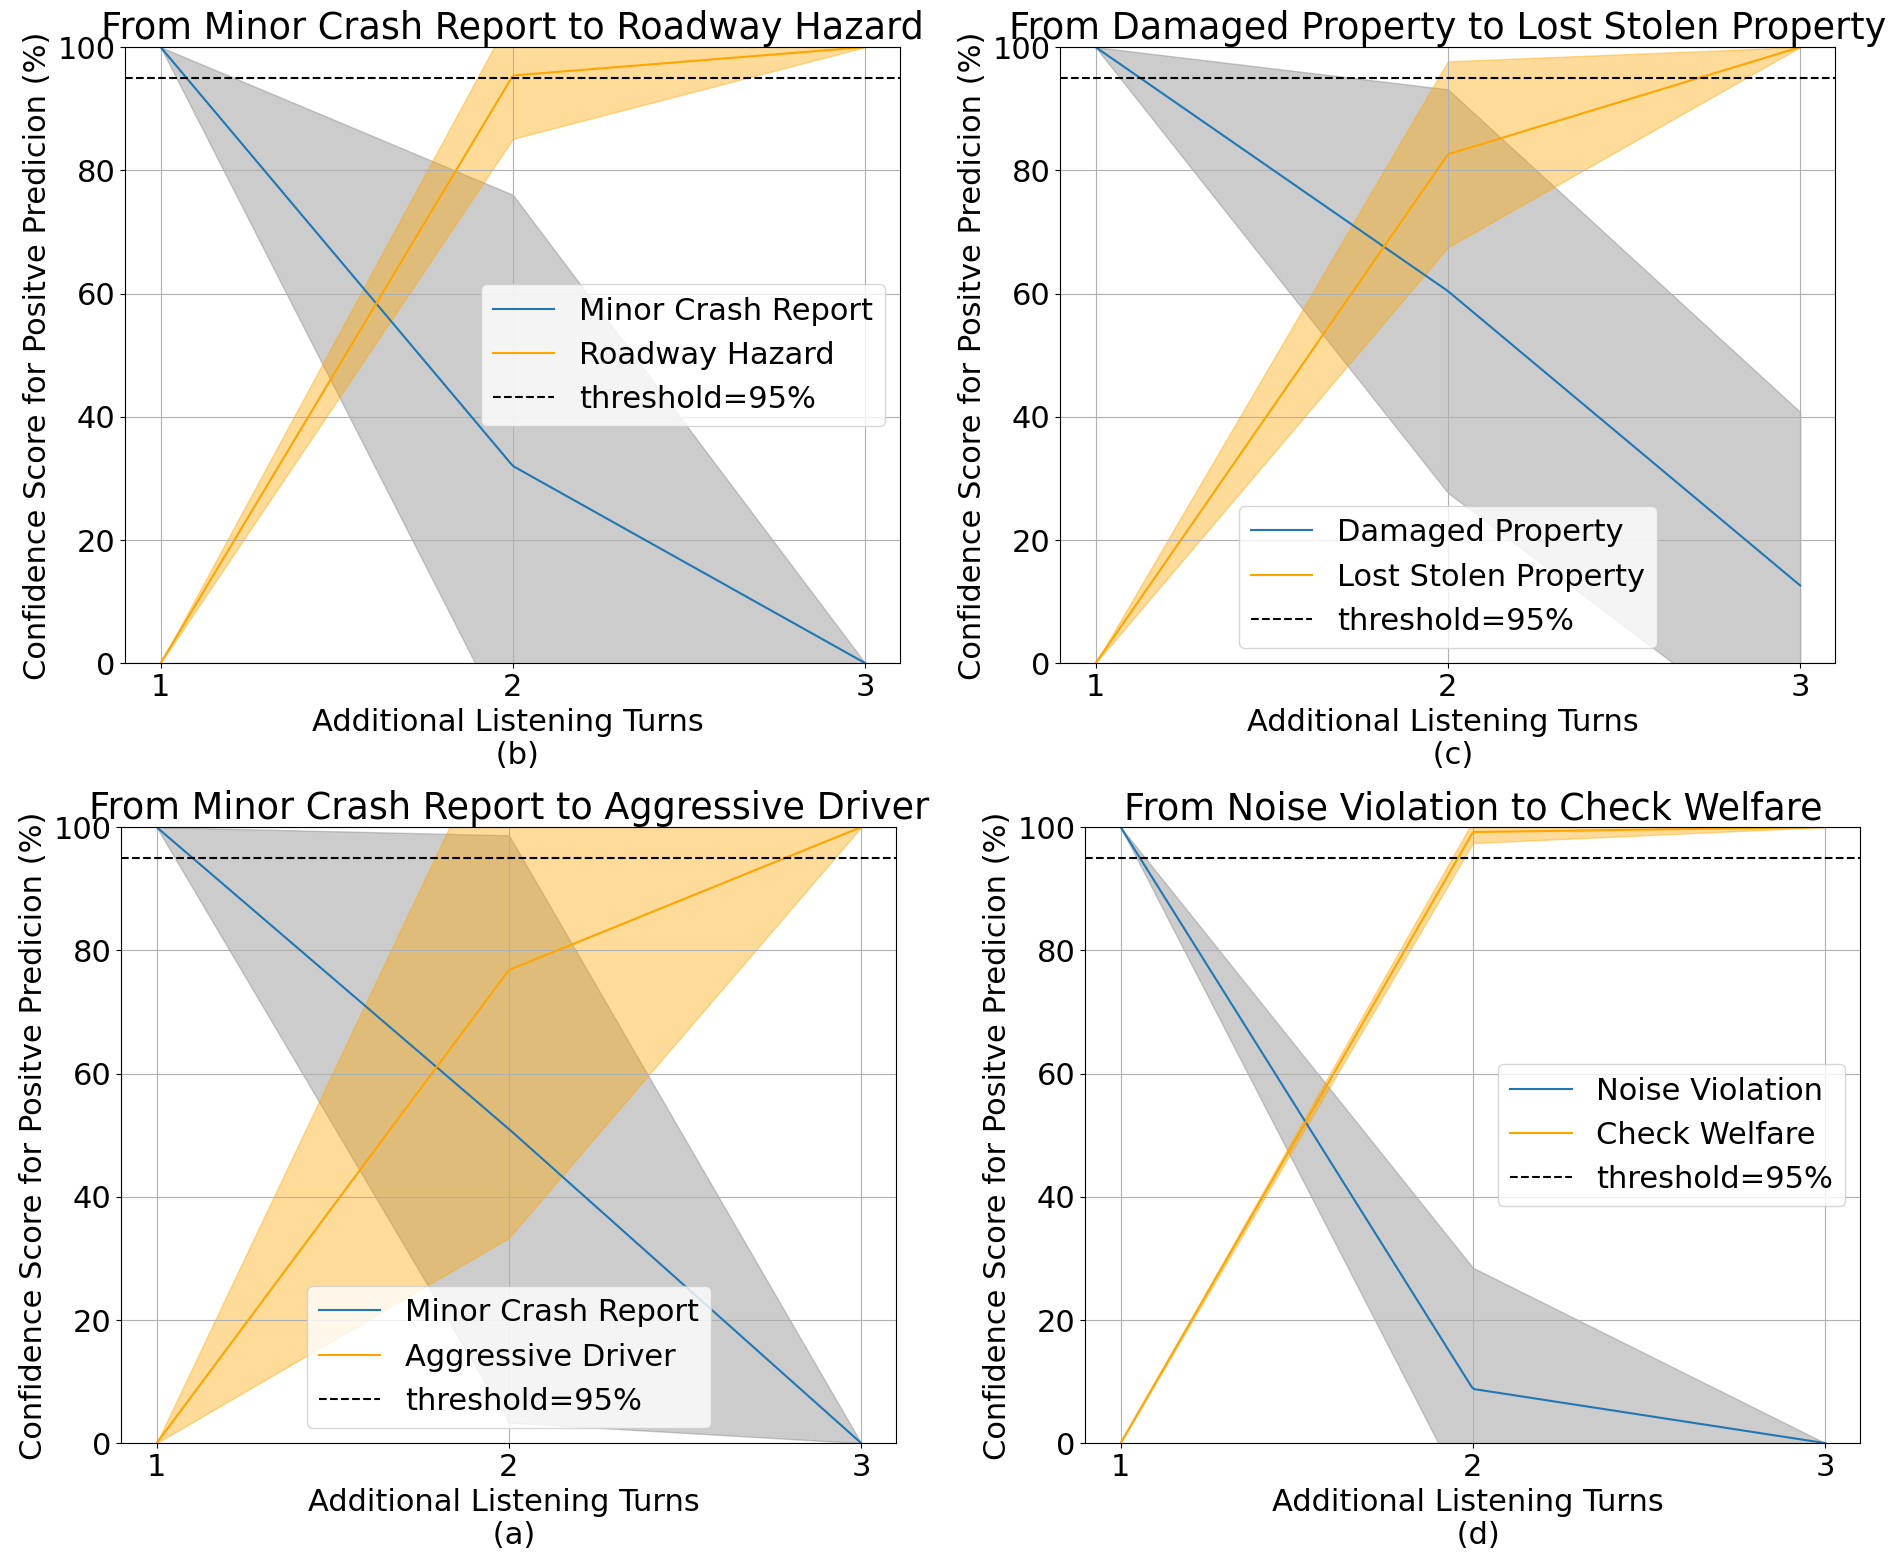
\includegraphics[width=0.40\textwidth]{figures/conf_curve.png}
    \caption{Confidence Changes in Shifting Incident Types}
    \label{fig:conf_curve}
    \vspace{-0.5cm}
\end{figure}

From Figure \ref{fig:conf_curve}, we observe that first, Auto311 handles all four major shifting situations in three future turns with more type-specific descriptions being fed as input to the incident type prediction module. Second, with the introduction of confidence guidance, Auto311 adjusts the prediction results to align with the shifting trend dynamically.

\textit{In summary, Auto311 adeptly handles shifting incident types in simulations, updating its understanding and creating optimized reports with more specific information over 3 follow-up turns.}

% \textit{In summary, based on our experimental results, Auto311 is capable of handling multiple incident types not only by statically accurately telling all the types but also by appropriately adjusting to shifting incident types with more specific information being fed in few follow-up turns.}

\subsubsection{Optimizations to Upcoming Dialogues}

We emulate Auto311 usage by composing caller utterances and assessing the relationship between saved turns and utterance size (see Figure \ref{fig:emulation}). Utterance size represents the count of past segments included. Across 100 emulations per size, we monitor saved turns and categorization accuracy. These experiments evaluate Auto311's ability to optimize dialogues through accumulated context and to make type predictions effectively.

% We emulate Auto311 usage by feeding composed caller utterances and analyzing turns saved versus utterance size (Figure \ref{fig:emulation}). Utterance size refers to the number of past segments in the composed utterance. Size $n$ means $n$ previous segments are included. In 100 emulations per size, we monitor dialogue turns saved by Auto311 and also the accuracy in categorizing the composed utterances. Experiments assess Auto311's ability to optimize upcoming dialogues by leveraging accumulating context and prediction accuracy.

% To demonstrate Auto311's ability to optimize upcoming dialogues, we emulate the process of the usage of Auto311 by feeding the composed caller utterance to Auto311. During emulation, we analyze the number of turns that can be saved in future conversations with respect to the size of the composed utterances (100 emulations for each size), see Figure \ref{fig:emulation}, and monitor Auto311's accuracy in categorizing the composed utterances. The utterance size refers to the number of utterance segments used in the composed utterance; size $n$ means there are $n$ previous utterance segments included in the composed utterances. 


Longer composed utterances contain more itemizable details. The blue line indicates Auto311's saved turns during emulation, while the light blue region represents total information provided. The average and maximum real-world utterance lengths are denoted by green and red dashed lines. Emulation demonstrates Auto311 effectively using additional information in caller utterances to minimize follow-up turns. Furthermore, Auto311 achieves a 94.49\% accuracy (not shown in Figure \ref{fig:emulation}) when handling composed utterances.

% Larger composed utterances contain more itemizable information. The blue line shows turns saved by Auto311 under emulation. The light blue region indicates the total information provided. Green and red dashed lines show average and maximum real-world utterance lengths. From the emulation, we find Auto311 is able to fully utilize the additional information conveyed in caller utterances to save follow-up turns. Additionally, Auto311 reports an overall accuracy of 94.49\% (not shown in Figure \ref{fig:emulation}) when faced with composed utterances.

% We observe that as the size of composed utterances gets larger, it contains more additional information for Auto311 to itemize. The blue line shows the turns saved by Auto311 under emulation. The light blue region indicates the amount of provided information based on current utterances. Green and red dashed lines indicate the average and maximum length of all the real-world caller utterances correspondingly. From the emulation, we find (1) Auto311 is able to fully utilize the additional information conveyed in caller utterances to save follow-up turns. Additionally, Auto311 reports an overall accuracy of 94.49\% when faced with composed utterances.


\begin{figure}[h]
    \centering
    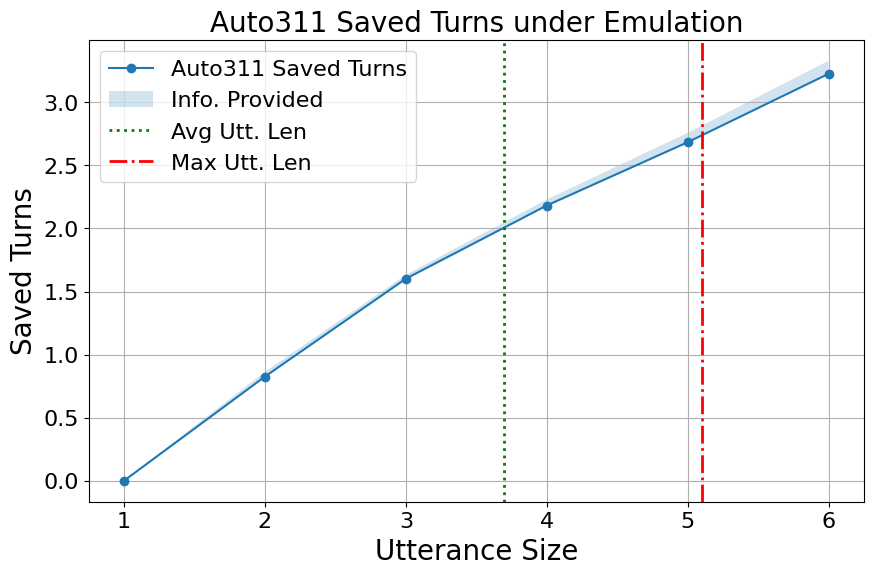
\includegraphics[width=0.40\textwidth]{figures/emulation.png}
    \caption{Emulated Usage of Auto311}
    \label{fig:emulation}
    \vspace{-0.5cm}
\end{figure}





% To demonstrate the impacts of our proposed system in real-world deployment, we simulate the working situation by emulating 10 random batches from the audio recordings to analyze (1) how many interactions can be potentially saved in further conversation based on the first few turns of dialogue and (2) how accurately can our system categorize the ongoing call. After our 10 emulations, with the assistance of our system, an average of 1.01 with a maximum of 1.86 turns can be theoretically reduced in future conversations based on the information provided in real audio recordings. Meanwhile, our system reports an overall accuracy of 94.49\% when dispatching the ongoing call to given incident types.

% \textit{In summary, the emulations demonstrate, at a system level, Auto311: (1) piratically optimizes future dialogues by fully utilizing additional utterance information. (2) effectively categorizes potential incident types with 94.49\% overall accuracy.}

\textit{In summary, these emulations prove our solution, at a system level, not only piratically optimizes future conversations by utilizing additional information provided in caller utterances but also effectively categorizes the potential incident types with an overall accuracy of 94.49\%.}

